% Options for packages loaded elsewhere
\PassOptionsToPackage{unicode}{hyperref}
\PassOptionsToPackage{hyphens}{url}
\PassOptionsToPackage{dvipsnames,svgnames,x11names}{xcolor}
%
\documentclass[
  letterpaper,
  DIV=11,
  numbers=noendperiod]{scrartcl}

\usepackage{amsmath,amssymb}
\usepackage{iftex}
\ifPDFTeX
  \usepackage[T1]{fontenc}
  \usepackage[utf8]{inputenc}
  \usepackage{textcomp} % provide euro and other symbols
\else % if luatex or xetex
  \usepackage{unicode-math}
  \defaultfontfeatures{Scale=MatchLowercase}
  \defaultfontfeatures[\rmfamily]{Ligatures=TeX,Scale=1}
\fi
\usepackage{lmodern}
\ifPDFTeX\else  
    % xetex/luatex font selection
\fi
% Use upquote if available, for straight quotes in verbatim environments
\IfFileExists{upquote.sty}{\usepackage{upquote}}{}
\IfFileExists{microtype.sty}{% use microtype if available
  \usepackage[]{microtype}
  \UseMicrotypeSet[protrusion]{basicmath} % disable protrusion for tt fonts
}{}
\makeatletter
\@ifundefined{KOMAClassName}{% if non-KOMA class
  \IfFileExists{parskip.sty}{%
    \usepackage{parskip}
  }{% else
    \setlength{\parindent}{0pt}
    \setlength{\parskip}{6pt plus 2pt minus 1pt}}
}{% if KOMA class
  \KOMAoptions{parskip=half}}
\makeatother
\usepackage{xcolor}
\setlength{\emergencystretch}{3em} % prevent overfull lines
\setcounter{secnumdepth}{-\maxdimen} % remove section numbering
% Make \paragraph and \subparagraph free-standing
\ifx\paragraph\undefined\else
  \let\oldparagraph\paragraph
  \renewcommand{\paragraph}[1]{\oldparagraph{#1}\mbox{}}
\fi
\ifx\subparagraph\undefined\else
  \let\oldsubparagraph\subparagraph
  \renewcommand{\subparagraph}[1]{\oldsubparagraph{#1}\mbox{}}
\fi

\usepackage{color}
\usepackage{fancyvrb}
\newcommand{\VerbBar}{|}
\newcommand{\VERB}{\Verb[commandchars=\\\{\}]}
\DefineVerbatimEnvironment{Highlighting}{Verbatim}{commandchars=\\\{\}}
% Add ',fontsize=\small' for more characters per line
\usepackage{framed}
\definecolor{shadecolor}{RGB}{241,243,245}
\newenvironment{Shaded}{\begin{snugshade}}{\end{snugshade}}
\newcommand{\AlertTok}[1]{\textcolor[rgb]{0.68,0.00,0.00}{#1}}
\newcommand{\AnnotationTok}[1]{\textcolor[rgb]{0.37,0.37,0.37}{#1}}
\newcommand{\AttributeTok}[1]{\textcolor[rgb]{0.40,0.45,0.13}{#1}}
\newcommand{\BaseNTok}[1]{\textcolor[rgb]{0.68,0.00,0.00}{#1}}
\newcommand{\BuiltInTok}[1]{\textcolor[rgb]{0.00,0.23,0.31}{#1}}
\newcommand{\CharTok}[1]{\textcolor[rgb]{0.13,0.47,0.30}{#1}}
\newcommand{\CommentTok}[1]{\textcolor[rgb]{0.37,0.37,0.37}{#1}}
\newcommand{\CommentVarTok}[1]{\textcolor[rgb]{0.37,0.37,0.37}{\textit{#1}}}
\newcommand{\ConstantTok}[1]{\textcolor[rgb]{0.56,0.35,0.01}{#1}}
\newcommand{\ControlFlowTok}[1]{\textcolor[rgb]{0.00,0.23,0.31}{#1}}
\newcommand{\DataTypeTok}[1]{\textcolor[rgb]{0.68,0.00,0.00}{#1}}
\newcommand{\DecValTok}[1]{\textcolor[rgb]{0.68,0.00,0.00}{#1}}
\newcommand{\DocumentationTok}[1]{\textcolor[rgb]{0.37,0.37,0.37}{\textit{#1}}}
\newcommand{\ErrorTok}[1]{\textcolor[rgb]{0.68,0.00,0.00}{#1}}
\newcommand{\ExtensionTok}[1]{\textcolor[rgb]{0.00,0.23,0.31}{#1}}
\newcommand{\FloatTok}[1]{\textcolor[rgb]{0.68,0.00,0.00}{#1}}
\newcommand{\FunctionTok}[1]{\textcolor[rgb]{0.28,0.35,0.67}{#1}}
\newcommand{\ImportTok}[1]{\textcolor[rgb]{0.00,0.46,0.62}{#1}}
\newcommand{\InformationTok}[1]{\textcolor[rgb]{0.37,0.37,0.37}{#1}}
\newcommand{\KeywordTok}[1]{\textcolor[rgb]{0.00,0.23,0.31}{#1}}
\newcommand{\NormalTok}[1]{\textcolor[rgb]{0.00,0.23,0.31}{#1}}
\newcommand{\OperatorTok}[1]{\textcolor[rgb]{0.37,0.37,0.37}{#1}}
\newcommand{\OtherTok}[1]{\textcolor[rgb]{0.00,0.23,0.31}{#1}}
\newcommand{\PreprocessorTok}[1]{\textcolor[rgb]{0.68,0.00,0.00}{#1}}
\newcommand{\RegionMarkerTok}[1]{\textcolor[rgb]{0.00,0.23,0.31}{#1}}
\newcommand{\SpecialCharTok}[1]{\textcolor[rgb]{0.37,0.37,0.37}{#1}}
\newcommand{\SpecialStringTok}[1]{\textcolor[rgb]{0.13,0.47,0.30}{#1}}
\newcommand{\StringTok}[1]{\textcolor[rgb]{0.13,0.47,0.30}{#1}}
\newcommand{\VariableTok}[1]{\textcolor[rgb]{0.07,0.07,0.07}{#1}}
\newcommand{\VerbatimStringTok}[1]{\textcolor[rgb]{0.13,0.47,0.30}{#1}}
\newcommand{\WarningTok}[1]{\textcolor[rgb]{0.37,0.37,0.37}{\textit{#1}}}

\providecommand{\tightlist}{%
  \setlength{\itemsep}{0pt}\setlength{\parskip}{0pt}}\usepackage{longtable,booktabs,array}
\usepackage{calc} % for calculating minipage widths
% Correct order of tables after \paragraph or \subparagraph
\usepackage{etoolbox}
\makeatletter
\patchcmd\longtable{\par}{\if@noskipsec\mbox{}\fi\par}{}{}
\makeatother
% Allow footnotes in longtable head/foot
\IfFileExists{footnotehyper.sty}{\usepackage{footnotehyper}}{\usepackage{footnote}}
\makesavenoteenv{longtable}
\usepackage{graphicx}
\makeatletter
\def\maxwidth{\ifdim\Gin@nat@width>\linewidth\linewidth\else\Gin@nat@width\fi}
\def\maxheight{\ifdim\Gin@nat@height>\textheight\textheight\else\Gin@nat@height\fi}
\makeatother
% Scale images if necessary, so that they will not overflow the page
% margins by default, and it is still possible to overwrite the defaults
% using explicit options in \includegraphics[width, height, ...]{}
\setkeys{Gin}{width=\maxwidth,height=\maxheight,keepaspectratio}
% Set default figure placement to htbp
\makeatletter
\def\fps@figure{htbp}
\makeatother

\KOMAoption{captions}{tableheading}
\makeatletter
\@ifpackageloaded{caption}{}{\usepackage{caption}}
\AtBeginDocument{%
\ifdefined\contentsname
  \renewcommand*\contentsname{Table of contents}
\else
  \newcommand\contentsname{Table of contents}
\fi
\ifdefined\listfigurename
  \renewcommand*\listfigurename{List of Figures}
\else
  \newcommand\listfigurename{List of Figures}
\fi
\ifdefined\listtablename
  \renewcommand*\listtablename{List of Tables}
\else
  \newcommand\listtablename{List of Tables}
\fi
\ifdefined\figurename
  \renewcommand*\figurename{Figure}
\else
  \newcommand\figurename{Figure}
\fi
\ifdefined\tablename
  \renewcommand*\tablename{Table}
\else
  \newcommand\tablename{Table}
\fi
}
\@ifpackageloaded{float}{}{\usepackage{float}}
\floatstyle{ruled}
\@ifundefined{c@chapter}{\newfloat{codelisting}{h}{lop}}{\newfloat{codelisting}{h}{lop}[chapter]}
\floatname{codelisting}{Listing}
\newcommand*\listoflistings{\listof{codelisting}{List of Listings}}
\makeatother
\makeatletter
\makeatother
\makeatletter
\@ifpackageloaded{caption}{}{\usepackage{caption}}
\@ifpackageloaded{subcaption}{}{\usepackage{subcaption}}
\makeatother
\ifLuaTeX
  \usepackage{selnolig}  % disable illegal ligatures
\fi
\usepackage{bookmark}

\IfFileExists{xurl.sty}{\usepackage{xurl}}{} % add URL line breaks if available
\urlstyle{same} % disable monospaced font for URLs
\hypersetup{
  pdftitle={BIOSTAT 724 - Homework 1},
  pdfauthor={Austin Allen},
  colorlinks=true,
  linkcolor={blue},
  filecolor={Maroon},
  citecolor={Blue},
  urlcolor={Blue},
  pdfcreator={LaTeX via pandoc}}

\title{BIOSTAT 724 - Homework 1}
\author{Austin Allen}
\date{}

\begin{document}
\maketitle

\subsection{Problem 1}\label{problem-1}

In answering a question on a multiple-choice test, a student either
knows the answer or guesses. Let p be the probability that the student
knows the answer and 1- p the probability that the student guesses.
Assume that a student who guesses at the answer will be correct with
probability 1/m, where m is the number of multiple-choice alternatives.
What is the conditional probability that a student knew the answer to a
question, given that he or she answered it correctly? What happens when
m is very large? What happens when p is close to 0?

\begin{quote}
Let's solve this using Baye's Theorem. First, it'll be helpful to define
some terms:

\begin{itemize}
\tightlist
\item
  \(P(\text{Knows}) = p\)
\item
  \(P(\text{Guess}) - 1 - p\)
\item
  \(P(\text{Correct | Guess}) = \frac{1}{m}\)
\item
  We want to know \(P(\text{Knows | Correct})\)
\end{itemize}
\end{quote}

\begin{align*}
P(\text{Knows | Correct}) &= \frac{P(\text{Correct | Knows})P(\text{Knows})}{P(\text{Correct | Knows})P(\text{Knows}) + P(\text{Correct | Guess})P(\text{Guess})}\\
&= \frac{(1)(p)}{(1)(p) + (\frac{1}{m})(1 - p)}\\
&= \frac{p}{p + \frac{1 - p}{m}}\\
\end{align*}

\begin{quote}
We can see from this result that as m gets arbitrarily large, the
denominator approaches p and the probability goes to 1. This aligns with
our intuition because a correct guess among a larger number of choices
would be less likely. Likewise, if p is close to 0, the probability is
also close to zero.
\end{quote}

\subsection{Problem 2}\label{problem-2}

Suppose urn H is filled with 40\% green balls and 60\% red balls, and
urn T is filled with 60\% green balls and 40\% red balls. Someone will
flip a coin and then select a ball from urn H or urn T depending on
whether the coin lands heads or tails, respectively. Let X be 1 or 0 if
the coin lands heads or tails, and let Y be 1 or 0 if the ball is green
or red.

\subsubsection{Part a}\label{part-a}

Write out the joint distribution of X and Y in a table.

\begin{Shaded}
\begin{Highlighting}[]
\CommentTok{\# | echo: false}
\ImportTok{import}\NormalTok{ pandas }\ImportTok{as}\NormalTok{ pd}

\CommentTok{\# Define the joint probability table}
\NormalTok{df }\OperatorTok{=}\NormalTok{ pd.DataFrame(}
\NormalTok{    \{}\DecValTok{0}\NormalTok{: [}\FloatTok{0.2}\NormalTok{, }\FloatTok{0.3}\NormalTok{], }\DecValTok{1}\NormalTok{: [}\FloatTok{0.3}\NormalTok{, }\FloatTok{0.2}\NormalTok{]\},}
\NormalTok{    index}\OperatorTok{=}\NormalTok{pd.Index([}\DecValTok{0}\NormalTok{, }\DecValTok{1}\NormalTok{], name}\OperatorTok{=}\StringTok{"Y"}\NormalTok{),}
\NormalTok{    columns}\OperatorTok{=}\NormalTok{pd.Index([}\DecValTok{0}\NormalTok{, }\DecValTok{1}\NormalTok{], name}\OperatorTok{=}\StringTok{"X"}\NormalTok{),}
\NormalTok{)}

\CommentTok{\# Add marginal probabilities}
\NormalTok{df[}\StringTok{"P(Y)"}\NormalTok{] }\OperatorTok{=}\NormalTok{ df.}\BuiltInTok{sum}\NormalTok{(axis}\OperatorTok{=}\DecValTok{1}\NormalTok{)  }\CommentTok{\# Row sums (marginal P(Y))}
\NormalTok{df.loc[}\StringTok{"P(X)"}\NormalTok{] }\OperatorTok{=}\NormalTok{ df.}\BuiltInTok{sum}\NormalTok{(axis}\OperatorTok{=}\DecValTok{0}\NormalTok{)  }\CommentTok{\# Column sums (marginal P(X))}

\CommentTok{\# Display the table}
\BuiltInTok{print}\NormalTok{(df)}
\end{Highlighting}
\end{Shaded}

\begin{verbatim}
X       0    1  P(Y)
Y                   
0     0.2  0.3   0.5
1     0.3  0.2   0.5
P(X)  0.5  0.5   1.0
\end{verbatim}

\subsubsection{Part b}\label{part-b}

Find E(Y). What is the probability that the ball is green?

\(E(Y) = \sum y\cdot f_Y(y)\). In our table, we see that Y can take on
two values, 0 and 1. We can use the marginal probability to find that
\(\sum y\cdot f_Y(y) = (0)(0.5) + (1)(0.5) = 0.5\). Thus,
\(P(\text{Ball is green}) = 0.5\).

\subsubsection{Part c}\label{part-c}

Find Var(Y\textbar X=0), Var(Y\textbar X=1) and Var(Y). Thinking of
variance as measuring uncertainty, explain intuitively why one of these
variances is larger than the others.

\begin{quote}
Intuitively, I would expect the variance of Y without any additional
information regarding X to be greater than either variances of Y given X
= 0 and X = 1. That is, I expect
\(max(Var(Y), Var(Y|X=0), Var(Y|X=1)) = Var(Y)\). My reasoning is that
knowing something about X reduces our uncertainty of Y. Let's see if I'm
correct.
\end{quote}

\[
\begin{align*}
Var(Y) &= \sum_{i = 1}^n (Y_i - E[Y])^2\cdot f(Y)\\
&= (0 -0.5)^2(0.5) + (1-0.5)^2(0.5)\\
&= 0.25\\
Var(Y|X=x) &= \sum_{i =1}^n (Y_i - E[Y | x])^2\cdot f(y|x)\\
E(Y|X=x) &= \sum_{i = 1}^nY_i\cdot f(y|x)\\
E(Y|X=0) &= (0)(0.4) + (1)(0.6)\\
&= 0.6\\
E(Y|X=1) &= (0)(0.6) + (1)(0.4)\\
&= 0.4\\
Var(Y|X=0) &= (0 - 0.6)^2(0.4) + (1 - 0.6)^2(0.6)\\
&= 0.24\\
Var(Y|X=1) &= (0 - 0.4)^2(0.6) + (1 - 0.4)^2(0.4)\\
&= 0.24\\
\end{align*}
\]

\begin{quote}
As I guessed, knowing something about X does reduce the uncertainty
around Y. We see that the conditional variances are both less than the
variance of Y, even if it is by a small amount.
\end{quote}

\subsubsection{Part d}\label{part-d}

Suppose you see that the ball is green. What is the probability that the
coin turned up tails?

\begin{quote}
Let's solve this in terms of X and Y. Thus, we want \(P(X=0|Y=1)\),
which is easily solved using Bayes' Theorem:
\end{quote}

\begin{align*}
P(X=0|Y=1) &= \frac{P(Y=1|X=0)P(X=0)}{P(Y=1|X=0)P(X=0) + P(Y=1|X=1)P(X=1)}\\
&= \frac{(0.6)(0.5)}{(0.6)(0.5) + (0.4)(0.5)}\\
&= 0.6
\end{align*}

\subsection{Problem 3}\label{problem-3}

Let \(\theta\) be a Beta(a,b) random variable, and suppose that the
conditional distribution of X, given that \(\theta\), is Binomial(n,
\(\theta\)). Find the (marginal) probability mass function of X.

\begin{quote}
We can solve this by integrating out \(\theta\) from the joint
distribution.
\end{quote}

\begin{align*}
f_X(X) &= \int P(X=x|\theta)P(\theta)d\theta\\
&= \int {n \choose x} \theta^x(1 - \theta)^{n - x}\theta^{a-1}(1-\theta)^{b-1}\frac{\Gamma(a + \beta)}{\Gamma(a)\Gamma(b)}d\theta\\
&= \int {n \choose x} \theta^{x+a-1}(1 - \theta)^{n + b- x-1}\frac{\Gamma(a + \beta)}{\Gamma(a)\Gamma(b)}d\theta\\
&= {n \choose x}\frac{\Gamma(a+b)}{\Gamma(a)\Gamma(b)} \int\theta^{x+a-1}(1 - \theta)^{n + b- x-1}d\theta\\
&= {n \choose x}\frac{\Gamma(a+b)}{\Gamma(a)\Gamma(b)}\frac{\Gamma(x + a - 1)\Gamma(b + n - x - 1)}{\Gamma(a + b + n - 2)}\int \theta^{x+a-1}(1 - \theta)^{n + b- x-1}d\theta \frac{\Gamma(a + b + n - 2)}{\Gamma(x + a - 1)\Gamma(b + n - x - 1)}d\theta\\
&= {n \choose x}\frac{\Gamma(a+b)}{\Gamma(a)\Gamma(b)}\frac{\Gamma(x + a - 1)\Gamma(b + n - x - 1)}{\Gamma(a + b + n - 2)} (1)\\
\end{align*}

\subsection{Problem 4}\label{problem-4}

Full conditionals: Let X,Y,Z be random variables with joint density
(discrete or continuous) p(x, y, z) ∝ f(x, z)g(y, z)h(z). Show that

\begin{enumerate}
\def\labelenumi{(\alph{enumi})}
\tightlist
\item
  p(x\textbar y, z) ∝ f(x, z), i.e.~, p(x\textbar y, z) is a function of
  x and z;
\item
  p(y\textbar x, z) \propto g(y, z), i.e., p(y\textbar x, z) is a
  function of y and z;
\item
  X and Y are conditionally independent given Z.
\end{enumerate}

\subsubsection{Part a}\label{part-a-1}

\begin{align*}
p(x|y, z) &= \frac{p(x, y, z)}{p(y)p(z)}\\
\implies p(x|y, z) &\propto p(x, y, z)\\
\implies p(x|y, z) &\propto f(x, z)g(y, z)h(z)\\
\end{align*}

\begin{quote}
Note that the only part of this that depends on X is \(f(x, z)\), which
implies that \(p(x|y, z) \propto f(x, z)\).
\end{quote}

\subsubsection{Part b}\label{part-b-1}

\begin{quote}
Let's solve this in the exact same way.
\end{quote}

\begin{align*}
p(y|x, z) &= \frac{p(x, y, z)}{p(x)p(z)}\\
\implies p(y|x, z) &\propto p(x, y, z)\\
\implies p(y|x, z) &\propto f(x, z)g(y, z)h(z)\\
\end{align*}

\begin{quote}
Similarly, the only portion of \(f(x, z)g(y, z)h(z)\) that depends on y
is the term \(g(y, z)\). Thus, \(p(y|x, z) \propto g(y, z)\).
\end{quote}

\subsubsection{Part c}\label{part-c-1}

\begin{quote}
To be conditionally independent, we need to show that
\(p(x, y|z) \propto p(x|z)p(y|z)\).

Let's begin with the same approach that we followed in parts a and b.
We'll obviously need to get a little fancier for this part, but let's
first show that \$p(x, y\textbar z) \propto f(x,z)g(y,z):
\end{quote}

\begin{align*}
p(y, x| z) &= \frac{p(x, y, z)}{p(z)}\\
\implies p(y,x| z) &\propto p(x, y, z)\\
\implies p(y,x| z) &\propto f(x, z)g(y, z)h(z)\\
\implies p(y,x| z) &\propto f(x, z)g(y, z)\\
\end{align*}

\begin{quote}
Next, we need to think about \(p(x|z)\) and \(p(y|z)\).
\end{quote}

\begin{align*}
p(x|z) &= \frac{p(x,z)}{p(z)}\\
p(x,z) \propto f(x,z)f(z)\\
\implies p(x|z)\propto f(x,z)\\
p(y|z) &= \frac{p(y,z)}{p(z)}\\
p(y,z) \propto g(y,z)f(z)\\
\implies p(y|z)\propto g(y,z)\\
\end{align*}

\begin{quote}
Combining these results, we see that
\(p(x, y | z)\propto f(x,z)g(y,z)\implies p(x, y |z) \propto p(x|z)p(y|z)\).
Thus, x and y are conditionally independent.
\end{quote}

\subsection{Part 5}\label{part-5}

PH 3.1

\subsubsection{Part a}\label{part-a-2}

Assume Y1, . . . , Y100 are, conditional on θ, i.i.d. binary random
variables with expectation θ. Write down the joint distribution of Pr(Y1
= y1, . . . , Y100 = y100\textbar θ) in a compact form. Also write down
the form of \(Pr(\sum PYi = y|θ)\).

\begin{align*}
f(y_1, ..., y_{100}|\theta) &= \prod_{i=1}^{100}f(y_i|\theta)\\
&= \theta^{\sum_{i = 1}^{100}y_i}(1 - \theta)^{n - \sum_{i = 1}^{100}y_i}\\
P\left(\sum_{i = 1}^{100}Y = y_i|\theta\right) &= {n \choose \sum y_i} \theta^{\sum y_i}(1 - \theta)^{n - \sum y_i}
\end{align*}

\subsubsection{Part b}\label{part-b-2}

For the moment, suppose you believed that θ ∈ \{0.0, 0.1, . . . , 0.9,
1.0\}. Given that the results of the survey were \(\sum Yi = 57\),
compute \(Pr(\sum Yi = 57|θ)\) for each of these 11 values of θ and plot
these probabilities as a function of θ.

\begin{Shaded}
\begin{Highlighting}[]
\DocumentationTok{\#\#\#\#\#\#\#\#\#\#\#\#\#\#\#\#\#\#\#\#\#\#\#\#\#\#\#\#\#\#\#\#\#\#\#\#\#\# R \#\#\#\#\#\#\#\#\#\#\#\#\#\#\#\#\#\#\#\#\#\#\#\#\#\#\#\#\#\#\#\#\#\#\#\#\#\#}
\FunctionTok{library}\NormalTok{(ggplot2)}

\CommentTok{\# Define a function that will spit out the probability we\textquotesingle{}re interested in}
\CommentTok{\# computing}
\NormalTok{p\_y\_theta }\OtherTok{\textless{}{-}} \ControlFlowTok{function}\NormalTok{(theta, n, y) \{}
    \CommentTok{\# y: a sum of bernouli trials}
    \CommentTok{\# theta: a vector of values between 0 and 1 (can be length 1)}
    \CommentTok{\# n: number of bernouli trials}
    \FunctionTok{return}\NormalTok{(}\FunctionTok{choose}\NormalTok{(n, y) }\SpecialCharTok{*}\NormalTok{ theta}\SpecialCharTok{**}\NormalTok{y }\SpecialCharTok{*}\NormalTok{ (}\DecValTok{1} \SpecialCharTok{{-}}\NormalTok{ theta)}\SpecialCharTok{**}\NormalTok{(n }\SpecialCharTok{{-}}\NormalTok{ y))}
\NormalTok{\}}

\CommentTok{\# Define our primary input values (theta) and other given values (n, y)}
\NormalTok{theta }\OtherTok{\textless{}{-}} \FunctionTok{seq}\NormalTok{(}\DecValTok{0}\NormalTok{, }\DecValTok{1}\NormalTok{, }\AttributeTok{length.out =} \DecValTok{11}\NormalTok{)}
\NormalTok{n }\OtherTok{\textless{}{-}} \DecValTok{100}
\NormalTok{y }\OtherTok{\textless{}{-}} \DecValTok{57}

\CommentTok{\# Figure out where the highest probability lies}
\NormalTok{max\_prob\_theta }\OtherTok{\textless{}{-}}\NormalTok{ theta[}
    \FunctionTok{which}\NormalTok{(}\FunctionTok{p\_y\_theta}\NormalTok{(theta, n, y) }\SpecialCharTok{==} \FunctionTok{max}\NormalTok{(}\FunctionTok{p\_y\_theta}\NormalTok{(theta, n, y)))}
\NormalTok{]}
\CommentTok{\# Plot the outputs as nice and pretty as possible}
\NormalTok{plot\_data }\OtherTok{\textless{}{-}} \FunctionTok{data.frame}\NormalTok{(}\AttributeTok{theta =}\NormalTok{ theta, }\AttributeTok{y =} \FunctionTok{p\_y\_theta}\NormalTok{(theta, n, y))}
\FunctionTok{ggplot}\NormalTok{(plot\_data, }\FunctionTok{aes}\NormalTok{(}\AttributeTok{x =}\NormalTok{ theta, }\AttributeTok{y =}\NormalTok{ y)) }\SpecialCharTok{+}
    \FunctionTok{geom\_point}\NormalTok{(}\AttributeTok{col =} \StringTok{"skyblue"}\NormalTok{, }\AttributeTok{size =} \DecValTok{2}\NormalTok{) }\SpecialCharTok{+}
    \FunctionTok{geom\_line}\NormalTok{(}\AttributeTok{col =} \StringTok{"skyblue"}\NormalTok{, }\AttributeTok{lwd =} \FloatTok{0.5}\NormalTok{, }\AttributeTok{lty =} \DecValTok{2}\NormalTok{) }\SpecialCharTok{+}
    \FunctionTok{geom\_vline}\NormalTok{(}\AttributeTok{xintercept =}\NormalTok{ max\_prob\_theta, }\AttributeTok{col =} \StringTok{"firebrick"}\NormalTok{, }\AttributeTok{lwd =} \DecValTok{1}\NormalTok{, }\AttributeTok{lty =} \DecValTok{2}\NormalTok{) }\SpecialCharTok{+}
    \FunctionTok{labs}\NormalTok{(}\AttributeTok{title =} \StringTok{"Pr(sum(Y) = 57 | theta)"}\NormalTok{, }\AttributeTok{x =} \StringTok{"Theta"}\NormalTok{, }\AttributeTok{y =} \StringTok{"Probability"}\NormalTok{) }\SpecialCharTok{+}
    \FunctionTok{theme\_bw}\NormalTok{() }\SpecialCharTok{+}
    \FunctionTok{theme}\NormalTok{(}
        \AttributeTok{text =} \FunctionTok{element\_text}\NormalTok{(}\AttributeTok{family =} \StringTok{"serif"}\NormalTok{),}
        \AttributeTok{plot.title =} \FunctionTok{element\_text}\NormalTok{(}\AttributeTok{hjust =} \FloatTok{0.5}\NormalTok{, }\AttributeTok{face =} \StringTok{"bold"}\NormalTok{, }\AttributeTok{size =} \DecValTok{14}\NormalTok{)}
\NormalTok{    )}
\end{Highlighting}
\end{Shaded}

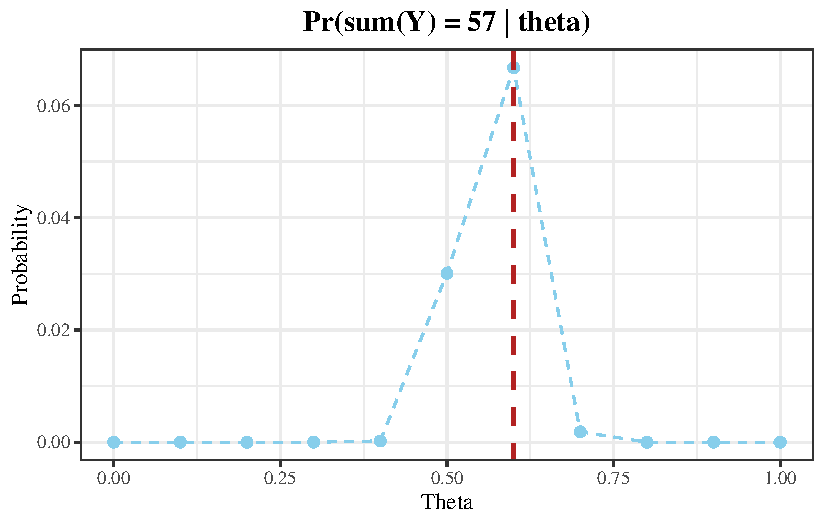
\includegraphics{hw2_files/figure-pdf/unnamed-chunk-2-1.pdf}

\begin{Shaded}
\begin{Highlighting}[]
\DocumentationTok{\#\#\#\#\#\#\#\#\#\#\#\#\#\#\#\#\#\#\#\#\#\#\#\#\#\#\#\#\#\#\#\#\#\#\#\#\#\#\#\#\#\#\#\#\#\#\#\#\#\#\#\#\#\#\#\#\#\#\#\#\#\#\#\#\#\#\#\#\#\#\#\#\#\#\#\#\#\#\#}
\end{Highlighting}
\end{Shaded}

\begin{quote}
The plot shows a maximum at 0.6.
\end{quote}

\subsubsection{Part c}\label{part-c-2}

Now suppose you originally had no prior information to believe one of
these θ-values over another, and so Pr(θ = 0.0) = Pr(θ = 0.1) = · · · =
Pr(θ = 0.9) = Pr(θ = 1.0). Use Bayes' rule to compute
\(p(θ| \sum Yi = 57)\) for each θ-value. Make a plot of this posterior
distribution as a function of θ.

\begin{quote}
I want to note that I used generative AI to assist me with the following
code for this problem. I derived the the math to implement, and ChatGPT
assisted with the coding:
\end{quote}

\begin{Shaded}
\begin{Highlighting}[]
\DocumentationTok{\#\#\#\#\#\#\#\#\#\#\#\#\#\#\#\#\#\#\#\#\#\#\#\#\#\#\#\#\#\#\#\#\#\#\#\#\#\# R \#\#\#\#\#\#\#\#\#\#\#\#\#\#\#\#\#\#\#\#\#\#\#\#\#\#\#\#\#\#\#\#\#\#\#\#\#\#}

\CommentTok{\# Define the function to compute posterior probability using Bayes\textquotesingle{} theorem}
\NormalTok{p\_theta\_bayes }\OtherTok{\textless{}{-}} \ControlFlowTok{function}\NormalTok{(theta, n, y) \{}
    \CommentTok{\# Compute P(Y = 57 | θ) for each θ}
\NormalTok{    likelihood }\OtherTok{\textless{}{-}} \FunctionTok{choose}\NormalTok{(n, y) }\SpecialCharTok{*}\NormalTok{ theta}\SpecialCharTok{\^{}}\NormalTok{y }\SpecialCharTok{*}\NormalTok{ (}\DecValTok{1} \SpecialCharTok{{-}}\NormalTok{ theta)}\SpecialCharTok{\^{}}\NormalTok{(n }\SpecialCharTok{{-}}\NormalTok{ y)}

    \CommentTok{\# Prior probabilities (uniform over 11 values)}
\NormalTok{    prior }\OtherTok{\textless{}{-}} \FunctionTok{rep}\NormalTok{(}\DecValTok{1} \SpecialCharTok{/} \FunctionTok{length}\NormalTok{(theta), }\FunctionTok{length}\NormalTok{(theta))}

    \CommentTok{\# Compute P(Y = 57) as the sum of likelihood * prior over all θ}
\NormalTok{    p\_y }\OtherTok{\textless{}{-}} \FunctionTok{sum}\NormalTok{(likelihood }\SpecialCharTok{*}\NormalTok{ prior)}

    \CommentTok{\# Compute posterior using Bayes\textquotesingle{} rule}
\NormalTok{    posterior }\OtherTok{\textless{}{-}}\NormalTok{ (likelihood }\SpecialCharTok{*}\NormalTok{ prior) }\SpecialCharTok{/}\NormalTok{ p\_y}

    \FunctionTok{return}\NormalTok{(posterior)}
\NormalTok{\}}

\CommentTok{\# Define theta values and known values of n and y}
\NormalTok{theta }\OtherTok{\textless{}{-}} \FunctionTok{seq}\NormalTok{(}\DecValTok{0}\NormalTok{, }\DecValTok{1}\NormalTok{, }\AttributeTok{length.out =} \DecValTok{11}\NormalTok{)}
\NormalTok{n }\OtherTok{\textless{}{-}} \DecValTok{100}
\NormalTok{y }\OtherTok{\textless{}{-}} \DecValTok{57}

\CommentTok{\# Compute the posterior probabilities}
\NormalTok{posterior\_probs }\OtherTok{\textless{}{-}} \FunctionTok{p\_theta\_bayes}\NormalTok{(theta, n, y)}

\CommentTok{\# Plot the posterior distribution}
\NormalTok{plot\_data }\OtherTok{\textless{}{-}} \FunctionTok{data.frame}\NormalTok{(}\AttributeTok{theta =}\NormalTok{ theta, }\AttributeTok{posterior =}\NormalTok{ posterior\_probs)}

\FunctionTok{ggplot}\NormalTok{(plot\_data, }\FunctionTok{aes}\NormalTok{(}\AttributeTok{x =}\NormalTok{ theta, }\AttributeTok{y =}\NormalTok{ posterior)) }\SpecialCharTok{+}
    \FunctionTok{geom\_point}\NormalTok{(}\AttributeTok{col =} \StringTok{"blue"}\NormalTok{, }\AttributeTok{size =} \DecValTok{2}\NormalTok{) }\SpecialCharTok{+}
    \FunctionTok{geom\_line}\NormalTok{(}\AttributeTok{col =} \StringTok{"blue"}\NormalTok{, }\AttributeTok{lwd =} \FloatTok{0.5}\NormalTok{, }\AttributeTok{lty =} \DecValTok{2}\NormalTok{) }\SpecialCharTok{+}
    \FunctionTok{labs}\NormalTok{(}
        \AttributeTok{title =} \StringTok{"Posterior Probability Distribution P(θ | Y = 57)"}\NormalTok{,}
        \AttributeTok{x =} \StringTok{"Theta"}\NormalTok{, }\AttributeTok{y =} \StringTok{"Posterior Probability"}
\NormalTok{    ) }\SpecialCharTok{+}
    \FunctionTok{theme\_bw}\NormalTok{() }\SpecialCharTok{+}
    \FunctionTok{theme}\NormalTok{(}
        \AttributeTok{text =} \FunctionTok{element\_text}\NormalTok{(}\AttributeTok{family =} \StringTok{"serif"}\NormalTok{),}
        \AttributeTok{plot.title =} \FunctionTok{element\_text}\NormalTok{(}\AttributeTok{hjust =} \FloatTok{0.5}\NormalTok{, }\AttributeTok{face =} \StringTok{"bold"}\NormalTok{, }\AttributeTok{size =} \DecValTok{14}\NormalTok{)}
\NormalTok{    )}
\end{Highlighting}
\end{Shaded}

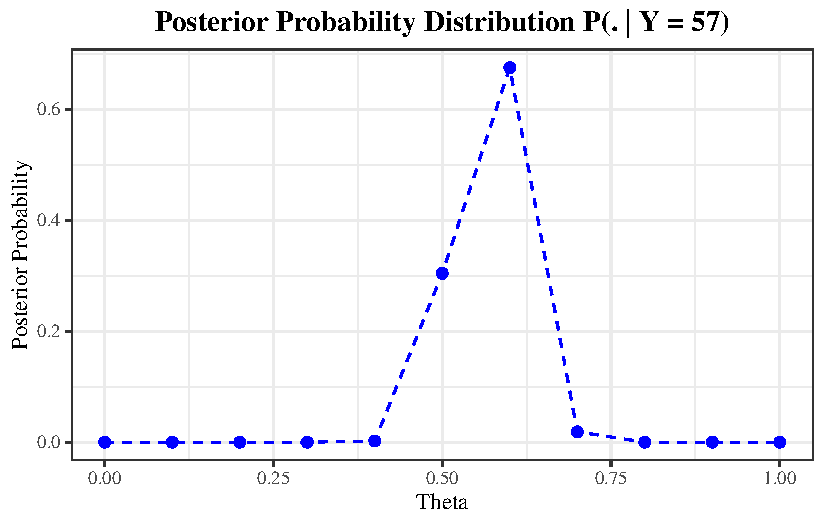
\includegraphics{hw2_files/figure-pdf/unnamed-chunk-3-1.pdf}

\begin{Shaded}
\begin{Highlighting}[]
\DocumentationTok{\#\#\#\#\#\#\#\#\#\#\#\#\#\#\#\#\#\#\#\#\#\#\#\#\#\#\#\#\#\#\#\#\#\#\#\#\#\#\#\#\#\#\#\#\#\#\#\#\#\#\#\#\#\#\#\#\#\#\#\#\#\#\#\#\#\#\#\#\#\#\#\#\#\#\#\#\#\#\#}
\end{Highlighting}
\end{Shaded}

\subsubsection{Part d}\label{part-d-1}

Now suppose you allow θ to be any value in the interval {[}0, 1{]}.
Using the uniform prior density for θ, so that p(θ) = 1, plot the
posterior density \(p(θ) × Pr(\sum Yi = 57|θ)\) as a function of θ.

\begin{Shaded}
\begin{Highlighting}[]
\DocumentationTok{\#\#\#\#\#\#\#\#\#\#\#\#\#\#\#\#\#\#\#\#\#\#\#\#\#\#\#\#\#\#\#\#\#\#\#\#\#\# R \#\#\#\#\#\#\#\#\#\#\#\#\#\#\#\#\#\#\#\#\#\#\#\#\#\#\#\#\#\#\#\#\#\#\#\#\#\#}
\FunctionTok{library}\NormalTok{(ggplot2)}

\CommentTok{\# Define function to compute posterior density}
\NormalTok{posterior\_density }\OtherTok{\textless{}{-}} \ControlFlowTok{function}\NormalTok{(theta\_vals, n, y) \{}
    \CommentTok{\# Compute likelihood P(Y = 57 | θ)}
\NormalTok{    likelihood }\OtherTok{\textless{}{-}} \FunctionTok{choose}\NormalTok{(n, y) }\SpecialCharTok{*}\NormalTok{ theta\_vals}\SpecialCharTok{\^{}}\NormalTok{y }\SpecialCharTok{*}\NormalTok{ (}\DecValTok{1} \SpecialCharTok{{-}}\NormalTok{ theta\_vals)}\SpecialCharTok{\^{}}\NormalTok{(n }\SpecialCharTok{{-}}\NormalTok{ y)}

    \CommentTok{\# Since prior is uniform (1), posterior is proportional to likelihood}
\NormalTok{    posterior }\OtherTok{\textless{}{-}}\NormalTok{ likelihood}

    \FunctionTok{return}\NormalTok{(posterior)}
\NormalTok{\}}

\CommentTok{\# Define a continuous range of theta values}
\NormalTok{theta\_vals }\OtherTok{\textless{}{-}} \FunctionTok{seq}\NormalTok{(}\DecValTok{0}\NormalTok{, }\DecValTok{1}\NormalTok{, }\AttributeTok{length.out =} \DecValTok{1000}\NormalTok{) }\CommentTok{\# More points for smooth curve}
\NormalTok{n }\OtherTok{\textless{}{-}} \DecValTok{100}
\NormalTok{y }\OtherTok{\textless{}{-}} \DecValTok{57}

\CommentTok{\# Compute posterior density}
\NormalTok{posterior\_vals }\OtherTok{\textless{}{-}} \FunctionTok{posterior\_density}\NormalTok{(theta\_vals, n, y)}

\CommentTok{\# Normalize for better visualization (optional, but makes y{-}axis interpretable)}
\NormalTok{posterior\_vals }\OtherTok{\textless{}{-}}\NormalTok{ posterior\_vals }\SpecialCharTok{/} \FunctionTok{max}\NormalTok{(posterior\_vals)}

\CommentTok{\# Plot the posterior density}
\NormalTok{plot\_data }\OtherTok{\textless{}{-}} \FunctionTok{data.frame}\NormalTok{(}\AttributeTok{theta =}\NormalTok{ theta\_vals, }\AttributeTok{posterior =}\NormalTok{ posterior\_vals)}

\FunctionTok{ggplot}\NormalTok{(plot\_data, }\FunctionTok{aes}\NormalTok{(}\AttributeTok{x =}\NormalTok{ theta, }\AttributeTok{y =}\NormalTok{ posterior)) }\SpecialCharTok{+}
    \FunctionTok{geom\_line}\NormalTok{(}\AttributeTok{col =} \StringTok{"skyblue"}\NormalTok{, }\AttributeTok{lwd =} \DecValTok{1}\NormalTok{) }\SpecialCharTok{+}
    \FunctionTok{labs}\NormalTok{(}
        \AttributeTok{title =} \StringTok{"Posterior Density p(θ | Y = 57)"}\NormalTok{,}
        \AttributeTok{x =} \StringTok{"Theta"}\NormalTok{, }\AttributeTok{y =} \StringTok{"Density (unnormalized)"}
\NormalTok{    ) }\SpecialCharTok{+}
    \FunctionTok{theme\_bw}\NormalTok{() }\SpecialCharTok{+}
    \FunctionTok{theme}\NormalTok{(}
        \AttributeTok{text =} \FunctionTok{element\_text}\NormalTok{(}\AttributeTok{family =} \StringTok{"serif"}\NormalTok{),}
        \AttributeTok{plot.title =} \FunctionTok{element\_text}\NormalTok{(}\AttributeTok{hjust =} \FloatTok{0.5}\NormalTok{, }\AttributeTok{face =} \StringTok{"bold"}\NormalTok{, }\AttributeTok{size =} \DecValTok{14}\NormalTok{)}
\NormalTok{    )}
\end{Highlighting}
\end{Shaded}

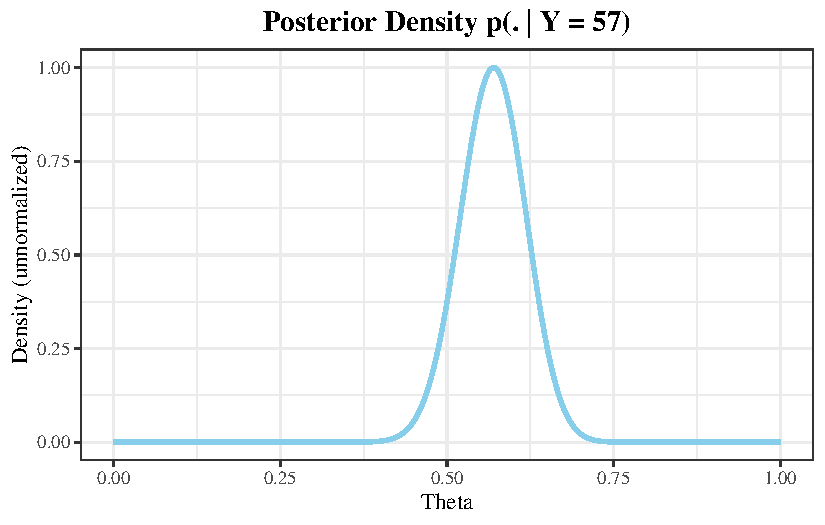
\includegraphics{hw2_files/figure-pdf/unnamed-chunk-4-1.pdf}

\begin{Shaded}
\begin{Highlighting}[]
\DocumentationTok{\#\#\#\#\#\#\#\#\#\#\#\#\#\#\#\#\#\#\#\#\#\#\#\#\#\#\#\#\#\#\#\#\#\#\#\#\#\#\#\#\#\#\#\#\#\#\#\#\#\#\#\#\#\#\#\#\#\#\#\#\#\#\#\#\#\#\#\#\#\#\#\#\#\#\#\#\#\#\#}
\end{Highlighting}
\end{Shaded}

\subsubsection{Part e}\label{part-e}

\begin{Shaded}
\begin{Highlighting}[]
\DocumentationTok{\#\#\#\#\#\#\#\#\#\#\#\#\#\#\#\#\#\#\#\#\#\#\#\#\#\#\#\#\#\#\#\#\#\#\#\#\#\# R \#\#\#\#\#\#\#\#\#\#\#\#\#\#\#\#\#\#\#\#\#\#\#\#\#\#\#\#\#\#\#\#\#\#\#\#\#\#}

\CommentTok{\# Define a function to return a posterior Beta(1+57, 1+100{-}57) density given}
\CommentTok{\# an input of theta values}
\NormalTok{posterior\_beta\_density }\OtherTok{\textless{}{-}} \ControlFlowTok{function}\NormalTok{(theta\_vals) \{}
    \FunctionTok{return}\NormalTok{(}\FunctionTok{dbeta}\NormalTok{(theta\_vals, }\DecValTok{1} \SpecialCharTok{+} \DecValTok{57}\NormalTok{, }\DecValTok{1} \SpecialCharTok{+} \DecValTok{100} \SpecialCharTok{{-}} \DecValTok{57}\NormalTok{))}
\NormalTok{\}}

\CommentTok{\# Get a set of density values like we did in part d}
\NormalTok{posterior\_probs }\OtherTok{\textless{}{-}} \FunctionTok{posterior\_beta\_density}\NormalTok{(theta\_vals)}

\CommentTok{\# Combine into a dataframe}
\NormalTok{plot\_data }\OtherTok{\textless{}{-}} \FunctionTok{data.frame}\NormalTok{(}\AttributeTok{theta =}\NormalTok{ theta\_vals, }\AttributeTok{density =}\NormalTok{ posterior\_probs)}

\CommentTok{\# Now let\textquotesingle{}s get back to plotting!}
\FunctionTok{ggplot}\NormalTok{(plot\_data, }\FunctionTok{aes}\NormalTok{(}\AttributeTok{x =}\NormalTok{ theta, }\AttributeTok{y =}\NormalTok{ density)) }\SpecialCharTok{+}
    \FunctionTok{geom\_line}\NormalTok{(}\AttributeTok{col =} \StringTok{"skyblue"}\NormalTok{, }\AttributeTok{lwd =} \DecValTok{1}\NormalTok{) }\SpecialCharTok{+}
    \FunctionTok{labs}\NormalTok{(}
        \AttributeTok{title =} \StringTok{"Posterior Density Beta(1+57, 100+1{-}57)"}\NormalTok{,}
        \AttributeTok{x =} \StringTok{"Theta"}\NormalTok{, }\AttributeTok{y =} \StringTok{"Density"}
\NormalTok{    ) }\SpecialCharTok{+}
    \FunctionTok{theme\_bw}\NormalTok{() }\SpecialCharTok{+}
    \FunctionTok{theme}\NormalTok{(}
        \AttributeTok{text =} \FunctionTok{element\_text}\NormalTok{(}\AttributeTok{family =} \StringTok{"serif"}\NormalTok{),}
        \AttributeTok{plot.title =} \FunctionTok{element\_text}\NormalTok{(}\AttributeTok{hjust =} \FloatTok{0.5}\NormalTok{, }\AttributeTok{face =} \StringTok{"bold"}\NormalTok{, }\AttributeTok{size =} \DecValTok{14}\NormalTok{)}
\NormalTok{    )}
\end{Highlighting}
\end{Shaded}

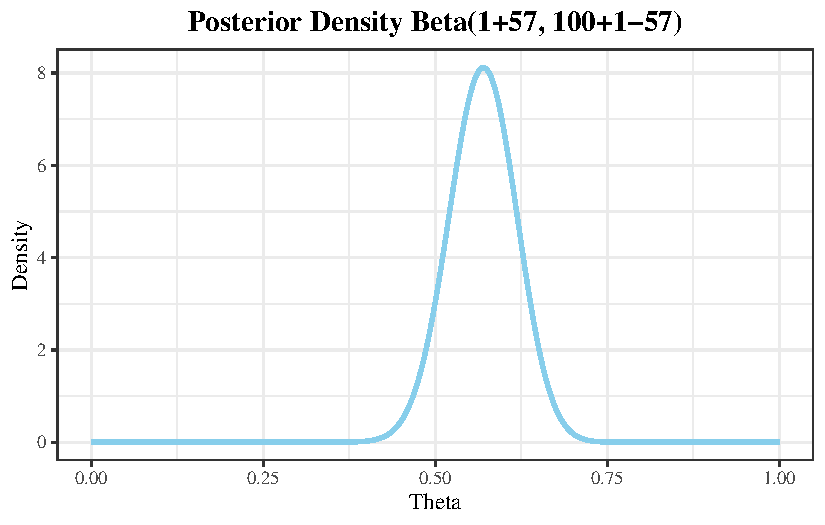
\includegraphics{hw2_files/figure-pdf/unnamed-chunk-5-1.pdf}

\begin{Shaded}
\begin{Highlighting}[]
\DocumentationTok{\#\#\#\#\#\#\#\#\#\#\#\#\#\#\#\#\#\#\#\#\#\#\#\#\#\#\#\#\#\#\#\#\#\#\#\#\#\#\#\#\#\#\#\#\#\#\#\#\#\#\#\#\#\#\#\#\#\#\#\#\#\#\#\#\#\#\#\#\#\#\#\#\#\#\#\#\#\#\#}
\end{Highlighting}
\end{Shaded}

\subsection{Part 6}\label{part-6}

PH 3.2



\end{document}
